\documentclass{article}
\usepackage[russian]{babel}
\usepackage[utf8]{inputenc}
\usepackage[T2]{fontenc}
\usepackage{graphicx}
\graphicspath{ {images/} }

\title{ТМП ДЗ №1}
\author{Максим Щемилкин A-05-19}
\date{30 марта 2022}

\begin{document}
\maketitle
\section{Построить конечный автомат, распознающий язык}


    \quad 1. $L = \{w \in \{a, b, c\}^*\quad|w|_c = 1\}$
    \begin{center}
        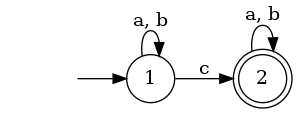
\includegraphics[width=0.4\textwidth]{pic1.dot}
    \end{center}
    \quad 2. $L = \{w \in \{a, b\}^* \quad |w|_a \leq 2, |w|_b \geq 2\}$
    \begin{center}
        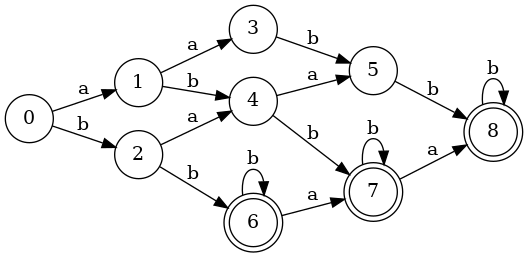
\includegraphics[width=0.8\textwidth]{pic2.dot}\\
    \end{center}
    Это решение получается через перебор первых 4 символов. Такой же результат можно получить через произведение двух грамматик:\\
    $$L_1 = \{w \in \{a, b\}^* \quad |w|_a \leq 2\}, \quad L_2 = \{w \in \{a, b\}^* \quad |w|_b \geq 2\}$$\\
    \begin{center}
        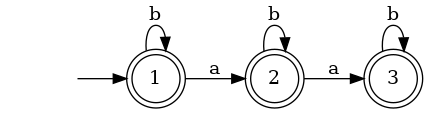
\includegraphics[width=0.45\textwidth]{pic3.dot}
        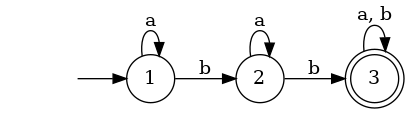
\includegraphics[width=0.45\textwidth]{pic4.dot}
    \end{center}
    \begin{center}
        \begin{tabular}{|c|c|c|}
            \hline
            Сочетания точек & По А & По В \\
            \hline
            11 & 21 & 12\\
            12 & 22 & 13\\
            13 & 23 & 13\\
            21 & 31 & 22\\
            22 & 32 & 23\\
            23 & 33 & 23\\
            31 &  & 32\\
            32 &  & 33\\
            33 &  & 33\\
            \hline
        \end{tabular}\\
    \end{center}
    Получим:
    \begin{center}
        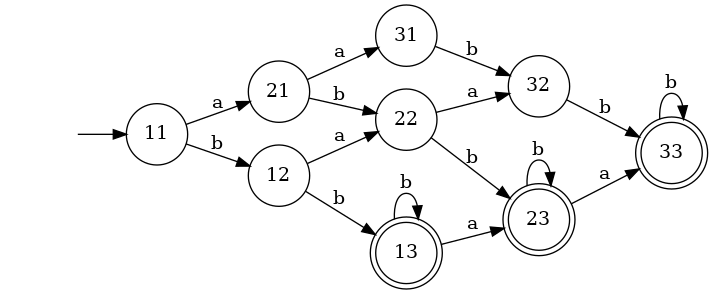
\includegraphics[width=0.9\textwidth]{pic5.dot}\\
    \end{center}
    \quad 3. $L = \{w \in \{a, b\}^* \quad |w|_a \neq |w|_b\}$
    \begin{center}
        Нет такого конечного автомата
    \end{center}
    \quad 4. $L = \{w \in \{a, b\}^* \quad ww = www\}$\\
    Это возможно только для языка, состоящего из пустого слова, так как при $|w|>0 ww \neq www$. Можем построить недерминированный КА:
    \begin{center}
        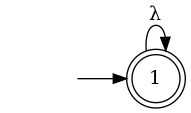
\includegraphics[width=0.3\textwidth]{pic6.dot}\\
    \end{center}
    
\section{Построить КА, используя прямое произведение}

    1. $L = \{w \in \{a, b\}^* \quad |w|_a \geq 2 \wedge |w|_b \geq 2\}$\\
    Разобьем на 2 автомата:
    $$L_1 = \{w \in \{a, b\}^* \quad |w|_a \geq 2\}, \quad L_2 = \{w \in \{a, b\}^* \quad |w|_b \geq 2\}$$\\
    \begin{center}
        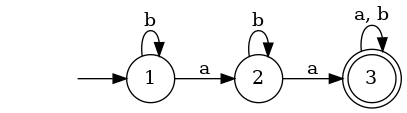
\includegraphics[width=0.45\textwidth]{pic7.dot}
        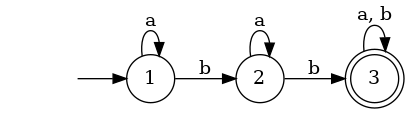
\includegraphics[width=0.45\textwidth]{pic4.dot}
    \end{center}
    Значит, $L = L_1 \wedge L_2$. Имеем $\Sigma = {a, b}, s = 11, T = 33$. Зафиксируем переходы между новыми вершинами:
    \begin{center}
        \begin{tabular}{|c|c|c|}
            \hline
            Сочетания точек & По А & По В \\
            \hline
            11 & 21 & 12\\
            12 & 22 & 13\\
            13 & 23 & 13\\
            21 & 31 & 22\\
            22 & 32 & 23\\
            23 & 33 & 23\\
            31 & 31 & 32\\
            32 & 32 & 33\\
            33 & 33 & 33\\
            \hline
        \end{tabular}\\
    \end{center}
    Получим:
    \begin{center}
        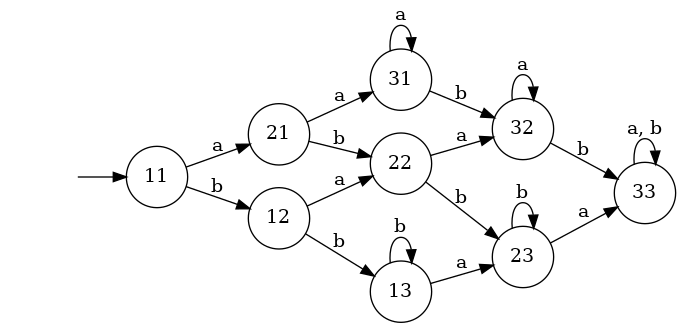
\includegraphics[width=0.9\textwidth]{pic8.dot}\\
    \end{center}
    
    2. $L = \{w \in \{a, b\}^* \quad |w| \geq 3 \wedge |w|\quad odd\}$\\
    Разобьем на 2 автомата:
    $$L_1 = \{w \in \{a, b\}^* \quad |w| \geq 3\}, \quad L_2 = \{w \in \{a, b\}^* \quad |w|\quad odd\}$$
    \begin{center}
        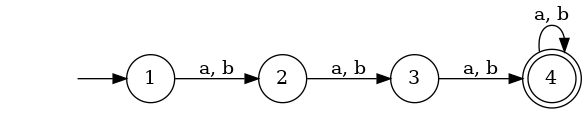
\includegraphics[width=0.6\textwidth]{pic9.dot}
        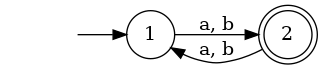
\includegraphics[width=0.3\textwidth]{pic10.dot}
    \end{center}
    Значит, $L = L_1 \wedge L_2$. Имеем $\Sigma = {a, b}, s = 11, T = 42$. Зафиксируем переходы между новыми вершинами:
    \begin{center}
        \begin{tabular}{|c|c|c|}
            \hline
            Сочетания точек & По А & По В \\
            \hline
            11 & 22 & 22\\
            12 & 21 & 21\\
            21 & 32 & 32\\
            22 & 31 & 31\\
            31 & 42 & 42\\
            32 & 41 & 41\\
            41 & 42 & 42\\
            42 & 41 & 41\\
            \hline
        \end{tabular}\\
    \end{center}
    Получим:
    \begin{center}
        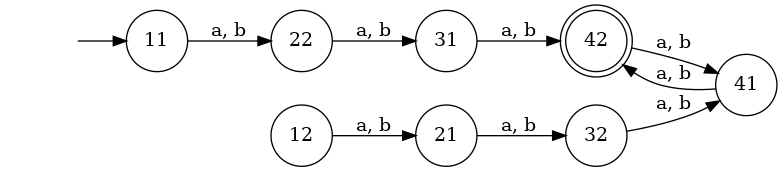
\includegraphics[width=0.9\textwidth]{pic11.dot}\\
    \end{center}
    Так как в вершину 12 попасть нельзя, можно автомат немного упростить:
    \begin{center}
        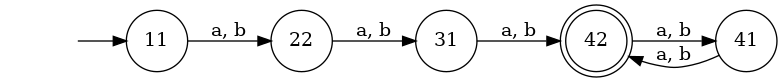
\includegraphics[width=0.9\textwidth]{pic12.dot}\\
    \end{center}
    
    3. $L = \{w \in \{a, b\}^* \quad |w|_a\, \vdots\, 2 \wedge |w|_b\, \vdots\, 3\}$\\
    Разобьем на 2 автомата:
    $$L_1 = \{w \in \{a, b\}^* \quad |w|_a\, \vdots\, 2\}, \quad L_2 = \{w \in \{a, b\}^* \quad |w|_b\, \vdots\, 3\}$$
    \begin{center}
        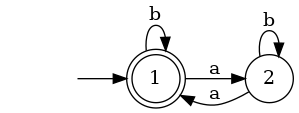
\includegraphics[width=0.4\textwidth]{pic13.dot}
        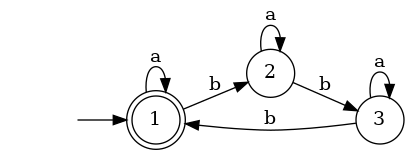
\includegraphics[width=0.5\textwidth]{pic14.dot}
    \end{center}
    Значит, $L = L_1 \wedge L_2$. Имеем $\Sigma = {a, b}, s = 11, T = 11$. Зафиксируем переходы между новыми вершинами:
    \begin{center}
        \begin{tabular}{|c|c|c|}
            \hline
            Сочетания точек & По А & По В \\
            \hline
            11 & 21 & 12\\
            12 & 22 & 13\\
            13 & 23 & 11\\
            21 & 11 & 22\\
            22 & 12 & 23\\
            23 & 13 & 21\\
            \hline
        \end{tabular}\\
    \end{center}
    Получим:
    \begin{center}
        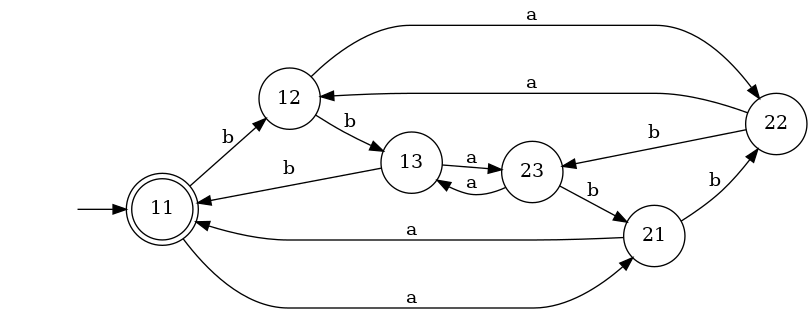
\includegraphics[width=0.9\textwidth]{pic15.dot}
    \end{center}
    
    
\end{document}
